% Introduction

The Python Computer Graphics Kit is a generic 3D package that can be
useful in any domain where you have to deal with 3D data of any kind,
be it for visualization, creating photorealistic images, Virtual Reality
or even games.

At its lowest level, the package provides the basic functionality that is
useful for writing your own tools that process 3D data. For example, the 
\module{cgtypes} module defines the fundamental types for Computer Graphics
such as vectors and matrices, the \module{ri} module contains the
complete RenderMan\textsuperscript{\textregistered} API to create RIB
files, and so on. Chapter \ref{modules1} documents all of these generic
modules.

Using these relatively low level modules the second level provides the
functionality to store a 3D scene in memory. This is the major part of
the package and this actually turns the general purpose language
Python into a specialized scripting language like MEL or MaxScript,
for example. 

Eventually, the package provides small tools that let you actually
{\em see} your 3D scene. The two standard tools are for interactive
rendering using OpenGL and for offline rendering using a 
RenderMan\textsuperscript{\textregistered} renderer.

%----------------------------------------------------------------------
\section{cgkit light}
\label{cgkitlight}

When the package is installed from the sources there is also the option
to install it as a 'light' version. The light version only consists of
pure Python modules and has no dependencies during installation. In
particular, you don't need a C/C++ compiler or any external library.
Some modules, such as \module{cgtypes}, that are actually implemented in C++
will be replaced by an alternative pure Python implementation so that
the functionality is still there, even though it will be less efficient.
This light version is meant to be used on any platform where the C++
support library and/or the wrapper modules cannot be compiled for whatever 
reasons and the setup script fails.

The downside of the light version, of course, is that you only get a 
fraction of the functionality from the full installation. Basically,
the light version exposes the general purpose modules from section
\ref{modules1} which comprises the functionality from version 1 of cgkit.

An attempt to import modules from the full installation will result
in an \exception{ImportError} exception.

The alternative pure Python implementations from the light version
are also available in the full installation in the \module{cgkit.light}
sub package. Usually you will not need this sub package, but there
might be situations where a pure Python implementation will have advantages
over a C++ implementation.


%----------------------------------------------------------------------
\section{External dependencies}
\label{externaldeps}

Some parts of this package make use of other external Python packages that
are not part of the standard Python installation. Whenever such functionality
is used the corresponding external package must be available or an exception
is raised. In general, the modules in cgkit try to delay such an exception
to the point where the respective package is actually {\em used} instead
of the time when it is imported. For example, you don't have to install
PyOpenGL, PIL or pygame if you only write command line tools that never
do a visualization.

The minimum requirement is, of course,
\ulink{Python}{http://www.python.org/} itself. The target Python
version is Python 2.3 and higher. However, some pure Python modules might also
run on earlier versions.

As long as only the general purpose modules (see chapter
\ref{modules1}) or the 'light' version of cgkit (see section
\ref{cgkitlight}) is used there is no external dependency.  If cgkit
is used to create and process a scene in memory then the following
packages might get used:

\begin{itemize}
\item \ulink{PyProtocols}{http://peak.telecommunity.com/PyProtocols.html}: This is a general requirement for scene management used in various places.
\item \ulink{numarray}{http://www.stsci.edu/resources/software_hardware/numarray}: This is mainly a requirement for PyOpenGL. At this time, cgkit itself does not use numarray yet.
\item \ulink{PyOpenGL}{http://pyopengl.sourceforge.net/}: This is only 
required when doing OpenGL visualizations, and even then it is only necessary
for some particular geometric objects (those that are implemented in Python).
As long as those objects aren't used (or are hidden) you can also do OpenGL
visualizations without PyOpenGL.
\item \ulink{PIL}{http://www.pythonware.com/products/pil/index.htm}: This is required whenever images have to be processed (such as for textures, for example).
\item \ulink{pygame}{http://www.pygame.org/}: This is only required when the viewer tool is used.
\end{itemize}

Some individual components might have other dependencies which is documented
on the respective page. However, as long as you don't use those components
you don't have to install the additional packages. So far, these are:

\begin{itemize}
\item \ulink{PyODE}{http://pyode.sourceforge.net/}: You need this if you want to do rigid body simulations using the \class{ODEDynamics} component.
\item \ulink{pySerial}{http://pyserial.sourceforge.net/}: You need this when you want to use the \code{FlockOfBirds} component.
\end{itemize}

%It might also be necessary to install the GLUT shared libraries 
%(\file{glut32.dll} on Windows) if they aren't already present on your system. 
%You can get them at \url{http://www.opengl.org}.

Windows: If you haven't already done so, it is recommended to add the
\file{Scripts} directory of your Python installation to your
\code{PATH} environment variable as this is the place where additional
tools are installed.

%----------------------------------------------------------------------
\section{An introductory tutorial}

This section gives a short introduction in the usage of the cgkit package.
In the first example, you create a simple scene that just has one
sphere (sort of a "Hello World" scene). To do so, create a file called
"helloworld.py" that contains the following line:

\begin{verbatim}
Sphere()
\end{verbatim}

Now launch the viewer tool passing the above file as argument (if you
have downloaded the source package, don't invoke the viewer tool from
inside the cgkit directory. If you do, Python will load the cgkit package
from the wrong directory and you'll get an ImportError exception):

\begin{verbatim}
> viewer.py helloworld.py
\end{verbatim}

The result should look something like this:

\begin{center}
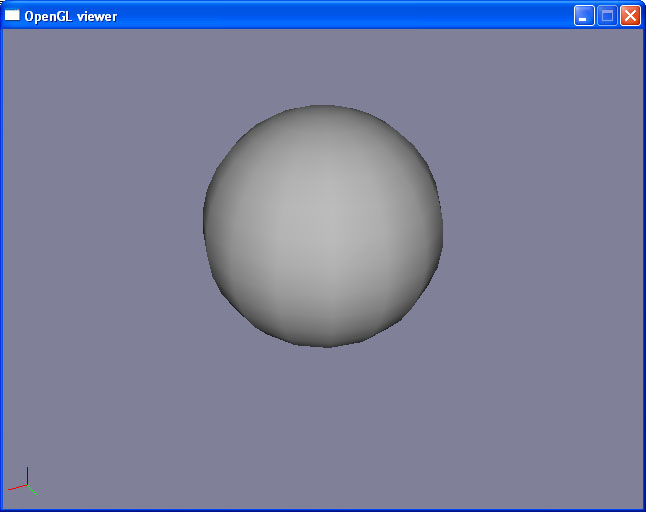
\includegraphics[width=8cm]{pics/helloworld}
\end{center}

The viewer tool reads the contents of the file which in this case
is an ordinary Python file and displays the scene using OpenGL.
When the input file is processed via the viewer tool it is executed
in a special environment where a couple of modules have already been imported.
That's why calling \code{Sphere()} doesn't result in a \exception{NameError}
exception. If you import the relevant modules yourself you can also call
the script without the viewer tool (however, you wouldn't get a visualization
of the scene then). You can also create the above scene directly in a 
Python shell:

\begin{verbatim}
>>> from cgkit.all import *
>>> Sphere()
<cgkit.quadrics.Sphere object at 0x051CC2D0>
\end{verbatim}

The first line imports all you need from cgkit which has to be done
manually now. The second line creates an instance of the
\class{Sphere} class. Usually, each object automatically inserts
itself into the scene, so we don't have to keep the resulting
reference. Now let's create another object:

\begin{verbatim}
>>> b=Box(name="Cube", pos=(1.5,2,0))
>>> listWorld()
Root
+---Cube (Box)
+---Sphere (Sphere)
\end{verbatim}

The first line creates a box object. This time we are passing a couple
of parameters like the object's name and its position and we store the
object in the variable \var{b} so we can manipulate the box afterwards.
The second line calls the \function{listWorld()} function
which prints a tree representation of the current scene.
Now it's time for a little nitpicking, actually the function only displays
the {\em world} (hence its name) and not the entire {\em scene}. The world
is what you see, it stores all 3D objects that have a visual representation
and is part of the scene. The whole scene also contains other objects
such as the timer, animation curves, etc. An object stored in the
scene is called a {\em component} and an object stored in the world
is, well, a {\em world object} (which is also a component as it is also
part of the scene). But back to the example. We have kept a reference to
the box, so let's see what we can do with it:

\begin{verbatim}
>>> b.name = "The Cube"
>>> listWorld()
Root
+---Sphere (Sphere)
+---The Cube (Box)
>>> b.pos
(1.5, 2, 0)
>>> b.pos=vec3(1,0,2)
>>> b.pos
(1, 0, 2)
>>> b.scale
(1, 1, 1)
\end{verbatim}

Every world object has a set of attributes that defines its state.
The exact set of attributes depends on the type of object, but there
are some common attributes that every world object has such as a name or
a position (see chapter \ref{worldobjects} for a reference of the available
world objects together with their attributes).

In the first example, we were only specifying one sphere with its default
attributes, that's why we had some geometry in the scene. But for a 3D scene
to be displayed you usually need two more ingredients: a camera and some 
light. In the above case, a default camera and light source was created
by the viewer tool. In the following example, we specify a complete scene,
including a camera, two colored light sources and a sphere with a material
assigned to it. Create a file "simplescene.py" with the following content:

\begin{verbatim}
TargetCamera(
    pos    = (3,2,2),
    target = (0,0,0)
)

GLPointLight(
    pos       = (3, -1, 2),
    diffuse   = (1, 0.7, 0.2)
)

GLPointLight(
    pos       = (-5, 3, 0),
    diffuse   = (0.2, 0.2, 0.5),
    intensity = 3.0
)

Sphere(
    name      = "My Sphere",
    radius    = 1.0,
    material  = GLMaterial(
                   diffuse = (0.7, 1, 0.7)
                )
)
\end{verbatim}

Display the scene by calling:

\begin{verbatim}
> viewer.py simplescene.py
\end{verbatim}

The result is this:

\begin{center}
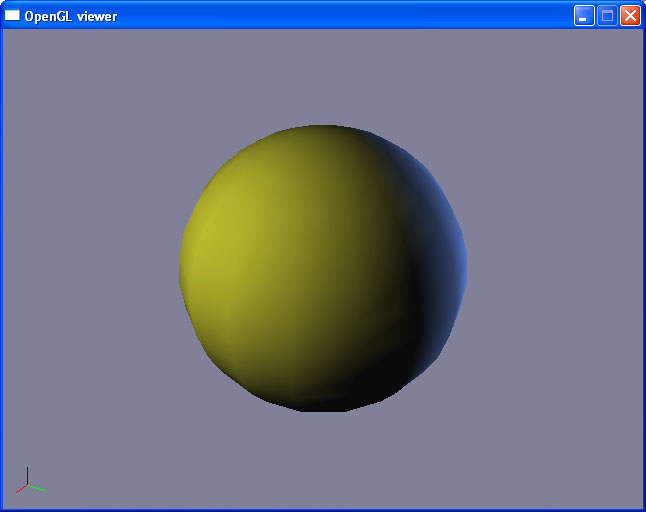
\includegraphics[width=8cm]{pics/simplescene1}
\end{center}

Using the \kbd{Alt} key in combination with the three mouse buttons
you can even navigate around in the scene (if you reach a pole
the camera position will jump around. This is because we are using
a \class{TargetCamera} that always tries to align its local "up"
direction with the global "up" direction, so this type of camera
can't be "upside down").

If you have a RenderMan renderer installed (there are free ones available
such as 3Delight, Aqsis or Pixie) you can try to visualize the above scene
with a different tool:

\begin{verbatim}
> render.py -r<renderer> simplescene.py
\end{verbatim}

\code{<renderer>} has to be replaced with either \code{3delight}, 
\code{aqsis} or \code{pixie}. 
This tool will display the same scene, but this time not using OpenGL but
the specified renderer. The result looks similar than before but is
much smoother:

\begin{center}
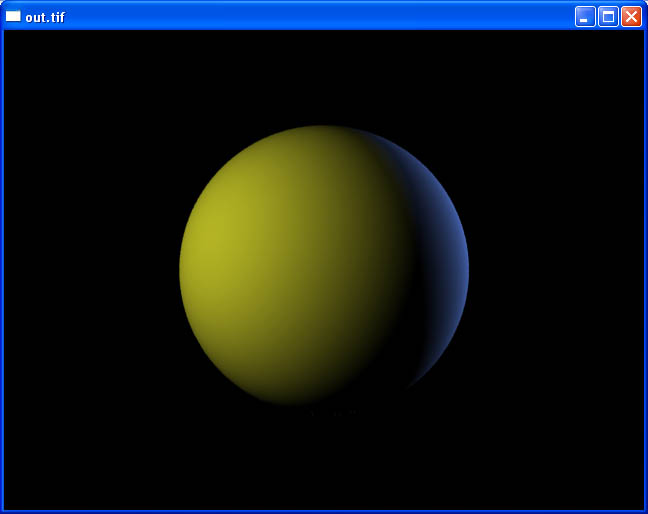
\includegraphics[width=8cm]{pics/simplescene2}
\end{center}

So if you want to create photorealistic images you can use the viewer tool
for previews and the render tool for creating the final image.

%----------------------------------------------------------------------
\section{Components and Slots}

This section gives an overview of the component framework that is the
basis for creating a dynamic 3D scene, i.e. one that is
animated/simulated. The basic mechanism is quite simple to understand
and you might already know it from other graphics packages as it is a
common concept in computer graphics software. The basic idea is to
have some black boxes that can generate values that vary with time and
that can be connected to the attributes we want to be animated. For
example, one such black box could output a three-dimensional vector
which could then be connected to the position of a teapot. If this
black box now produces a series of values that lie on a particular
curve we have an animation of a teapot traveling along that curve.

\begin{center}
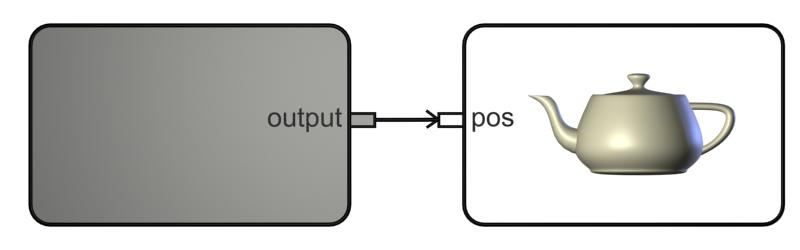
\includegraphics[width=10cm]{pics/slotexample}
\end{center}

In this package those black boxes and the teapot are called {\em
components}. A component is a container for {\em slots} which
represent the input or output values of their respective component. In
the above example, the output value of the "curve point generator" and
the position of the teapot are slots. You can also view them as
"animatable attributes" of an object if they mainly serve as input
values. Most slots can either serve as input value or output
value. However, if the value of a slot is actually computed by some
algorithm then this slot can only be used as output slot.

As a general rule, the actual slot corresponding to an attribute is
obtained by adding the suffix \code{_slot} to the attribute name.
Here is an example where two spheres s1 and s2 are created and
the position of s1 is connected to the position of s2 which means
s2 will always have the same position as s1:

\begin{verbatim}
>>> from cgkit import *
>>> s1=Sphere(pos=(1,2,3))
>>> s2=Sphere(pos=(-1,0,5))
>>> s1.pos
(1, 2, 3)
>>> s2.pos
(-1, 0, 5)

# Connect the positions 
>>> s1.pos_slot.connect(s2.pos_slot)

# Now s2 has the same position as s1
>>> s2.pos
(1, 2, 3)

# Changing the position of s1 will also change the position of s2
>>> s1.pos=vec3(-5,12,42)
>>> s2.pos
(-5, 12, 42)
\end{verbatim}

%----------------------------------------------------------------------
\section{Coordinate systems}

Each world object has a position and orientation in space. This
transformation can be described by a matrix that represents the
object's local coordinate system. The local coordinate system L stored
in each world object is given with respect to its parent coordinate
system which usually is just the world coordinate system unless you
have linked two objects. If you want the local coordinate system with
respect to the world system you have to travel up the transformation
hierarchy and concatenate all local systems (however, you don't have to
do that yourself as a world object already has an attribute 
\var{worldtransform} which does this for you). 

The geometry of a world object is given with respect to the local
coordinate system L. So this is the matrix that's required during
rendering. You get L by calling \method{localTransform()} on the
respective world object.

So far, if you would apply a rotation to an object it would rotate
around the origin or if you would scale the object the center of the
scale would lie in the origin. This is not always the desired behavior
and that's why you can specify a pivot point, or rather, a pivot
transformation or offset transformation P. This transformation is
given with respect to L and is the identity by default. You can get
and set this transformation using the \method{getOffsetTransform()} and
\method{setOffsetTransform()} methods.

The concatenation of L and P is the transformation T ($T=L\cdot
P$). This is what the
\var{transform}, \var{pos}, \var{rot} and \var{scale} slots of a world 
object describe. So if you modify the transform slot you also modify L
whereas P always remains constant, unless you change it explicitly via
\method{setOffsetTransform()}.

\begin{center}
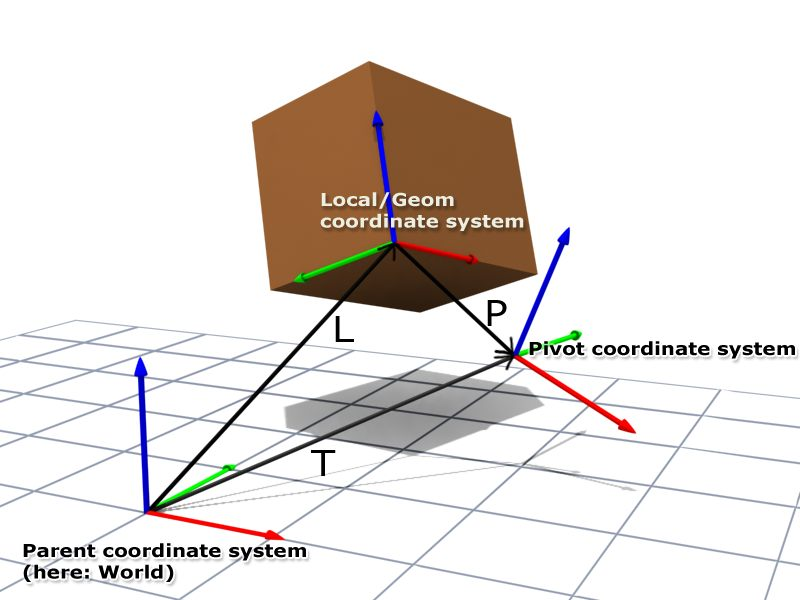
\includegraphics[width=12cm]{pics/coordsys}
\end{center}

Here is a simple code example where you can see the effects when
modifying the different transformations:

\begin{verbatim}
>>> s = Sphere()
>>> s.pos = vec3(1,2,0)
>>> s.pos
<1, 2, 0>
>>> s.setOffsetTransform(mat4().translation(vec3(2,4,7)))
>>> s.pos
<3, 6, 7>
>>> s.pos = vec3(0,0,0)
>>> s.pos
<0, 0, 0>
>>> s.localTransform()
[1, 0, 0, -2]
[0, 1, 0, -4]
[0, 0, 1, -7]
[0, 0, 0, 1]
\end{verbatim}